\documentclass[dvipdfmx]{jsarticle}


\usepackage{tcolorbox}
\usepackage{color}
\usepackage{listings, plistings}

%% ノート/latexメモ
%% http://pepper.is.sci.toho-u.ac.jp/pepper/index.php?%A5%CE%A1%BC%A5%C8%2Flatex%A5%E1%A5%E2

% Java
\lstset{% 
  frame=single,
  backgroundcolor={\color[gray]{.9}},
  stringstyle={\ttfamily \color[rgb]{0,0,1}},
  commentstyle={\itshape \color[cmyk]{1,0,1,0}},
  identifierstyle={\ttfamily}, 
  keywordstyle={\ttfamily \color[cmyk]{0,1,0,0}},
  basicstyle={\ttfamily},
  breaklines=true,
  xleftmargin=0zw,
  xrightmargin=0zw,
  framerule=.2pt,
  columns=[l]{fullflexible},
  numbers=left,
  stepnumber=1,
  numberstyle={\scriptsize},
  numbersep=1em,
  language={Java},
  lineskip=-0.5zw,
  morecomment={[s][{\color[cmyk]{1,0,0,0}}]{/**}{*/}},
  keepspaces=true,         % 空白の連続をそのままで
  showstringspaces=false,  % 空白字をOFF
}
%\usepackage[dvipdfmx]{graphicx}
\usepackage{url}
\usepackage[dvipdfmx]{hyperref}
\usepackage{amsmath, amssymb}
\usepackage{itembkbx}
\usepackage{eclbkbox}	% required for `\breakbox' (yatex added)
\usepackage{enumerate}
\fboxrule=0.5pt
\parindent=1em
\begin{document}

%\anaumeと入力すると穴埋め解答欄が作れるようにしてる。\anaumesmallで小さめの穴埋めになる。
\newcounter{mycounter} % カウンターを作る
\setcounter{mycounter}{0} % カウンターを初期化
\newcommand{\anaume}[1][]{\refstepcounter{mycounter}{#1}{\boxed{\phantom{aa}\themycounter \phantom{aa}}}} %穴埋め問題の空欄作ってる。
\newcommand{\anaumesmall}[1][]{\refstepcounter{mycounter}{#1}{\boxed{\tiny{\phantom{a}\themycounter \phantom{a}}}}}%小さい版作ってる。色々改造できる。

%% 修正時刻: Tue May  5 10:19:29 2020


\section{Telnetで GETリクエスト}

\subsection{ブラウザのやっていること}

現在、\textsf{test} フォルダを公開フォルダとして Webサーバーが動作している。

ブラウザから \textsf{http://localhost:8888} とすると、このフォルダにある
\textsf{index.html} を表示させることができる。

このとき、ブラウザはWebサーバーにどういう働きかけをしているのか?

また、Webサーバーはどういう返答をしているのか?

ブラウザのやっていることを \textsf{Telnet} でやってみることができる。

\subsection{GETリクエスト}

ブラウザから、あるサイトにアクセスして、そのページを表示させたいとする。

これをあるがままに言うと、ブラウザがあるサイトにアクセスして、

\framebox[10cm][c]{このページのHTMLをダウンロードさせてくれ}

という要求をおこなっていることになる。

これを \textgt{GETリクエスト} という。

\textgt{GETリクエスト} のやり方は決っていて、以下のようなコマンドを送る。

\begin{tcolorbox}
 \verb!GET / HTTP/1.1! \\
 \verb!Host: localhost:8888! \\
 (空行)
\end{tcolorbox}

1行目は、GETリクエストであることを示す。 
``/'' は、パスをあらわす。''/index.html'' を指定したことと同じ。 
''HTTP.1.1'' は、HTTPの1.1バージョンで通信するという意味。

2行目は、相手ホスト名を指定している。
80番ポート(普通はこのポート) なら省略できるが、我々はさきほど、このWebサーバーを
8888番ポートで起動したから、このポートを指定している。

そして、3行目は、\textgt{空行} を送る。これは絶対必要。

最後に $<$Enter$>$ を送る。

この空行までを\textgt{ヘッダ部}という。これが GETリクエストの決まりである。

これを TeraTerm でやってみる。

\subsection{TeraTermでGetリクエスト}

TeraTerm を起動する。

``ホスト'' に \textsf{localhost} と指定する。

``サービス'' は \textsf{Telnet} にチェックを入れる。

''TCPポート'' は \textsf{8888} と指定する。

ほかはそのままで、``OK''とする。

\vspace{3mm}
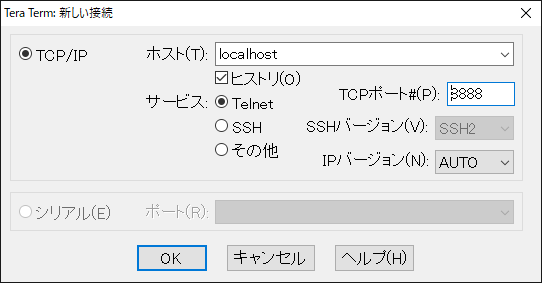
\includegraphics{../img/25-get-01.png}
\vspace{3mm}

黒い画面があらわれるので、以下の内容を黒い画面に入力する。

\begin{tcolorbox}
 \verb!GET / HTTP/1.1! \\
 \verb!Host: localhost:8888! \\
 (空行)
\end{tcolorbox}

大文字、小文字に気をつけて入力する。

\vspace{3mm}
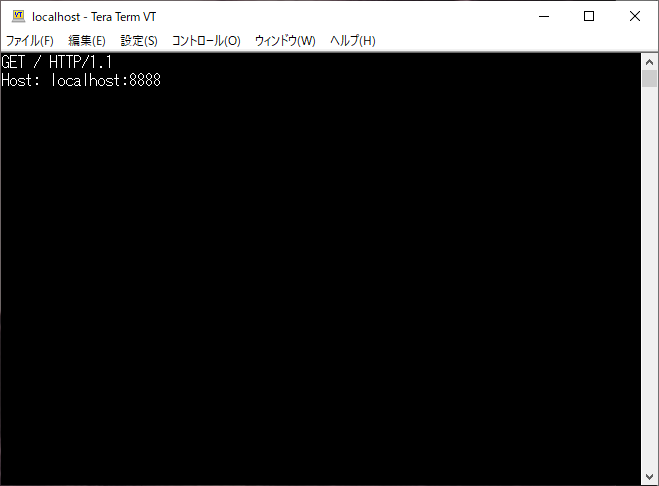
\includegraphics[width=14cm]{../img/26-get-02.png}
\vspace{3mm}

そして $<$Enter$>$ キーを押すと、以下のように出力される。

\vspace{3mm}
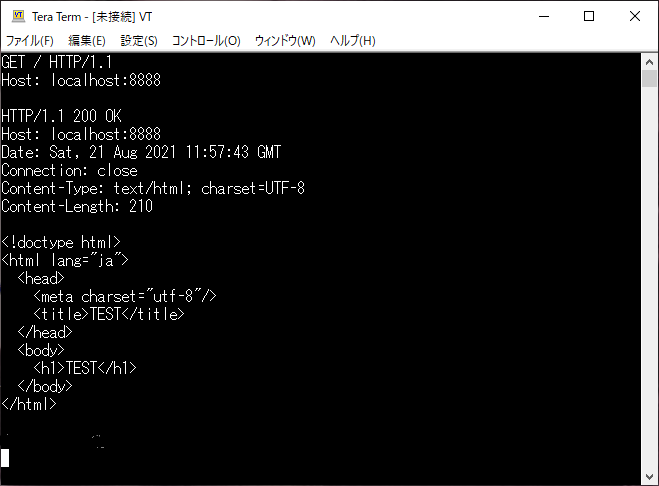
\includegraphics[width=14cm]{../img/27-get-03.png}
\vspace{3mm}

空行の下の ``HTTP...''以下は Webサーバーからの応答(レスポンス)である。

\begin{itemize}
 \item \textsf{HTTP/1.1} --- HTTPプロトコルのバージョン1.1 で応答するということ。
 \item \textsf{200 OK} ---  正常な処理だということ。
 \item \textsf{Host: localhost:8888} --- サーバー側のホスト名とポート番号。
 \item 日付 -- ''\textsf{GMT}'' となっているのは、グリニッジ標準時のこと。日本よりも9時間遅い。
 \item \textsf{Connection: close} --- この応答で接続が閉じられたことを表す。
 \item \textsf{Content-Type: text/html; charset=UTF-8} --- 空行の後に送る文字列(ボディ部)は
 HTMLで、文字コードは UTF-8 であることを (ブラウザに) 伝えている。
 \item \textsf{Content-Length: 210} --- 空行の後に送る文字列は 210文字であることを示している。\\
※ 210文字というのは、本当は 159文字で、この画像では消しているが、$<$/html$>$ の後に注釈の
文字列が続いていたのである。
\end{itemize}

ここまでが ''\textgt{ヘッダ部}'' で、''\textsf{空行}'' に区切られて、以下 ''\textsf{ボディ部}''が
続く。

ボディ部はブラウザが受け取って処理をする。つまり、文字や画像をブラウザの画面に表示するのである。
それを \textsf{レンダリング(描画)} という。

\subsection{さまざまな GET リクエスト}

Webサーバーに送る GET リクエストでは、``/'' のみを指定したが、それ以外にたとえば、``/menu.html''
などとファイル名(パス)を指定することが多い。

もし、存在しないファイル名を指定すると、どうなるか?

これは、存在しないファイル ''about.html'' を指定した例である。

\vspace{3mm}
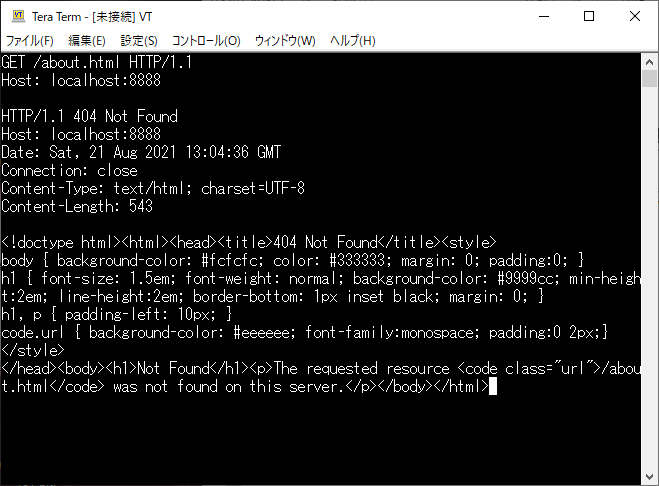
\includegraphics[width=15cm]{../img/28-not-found.png}
\vspace{3mm}

サーバーからの応答の1行目に、

\begin{tcolorbox}
 HTTP/1.1 404 Not Found
\end{tcolorbox}

とある。''404エラー'' と呼ばれる応答例である。
これをブラウザで表示すると、以下のようになる。

\vspace{3mm}
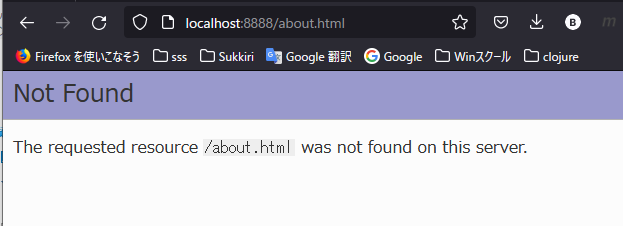
\includegraphics[width=10cm]{../img/29-not-found-2.png}
\vspace{3mm}




\end{document}

%% 修正時刻: Sat May  2 15:10:04 2020


%% 修正時刻: Sat Aug 21 22:14:32 2021
